  \subfloat[]{
    \begin{tikzpicture}[remember picture]
      \node[anchor=south west] (img) {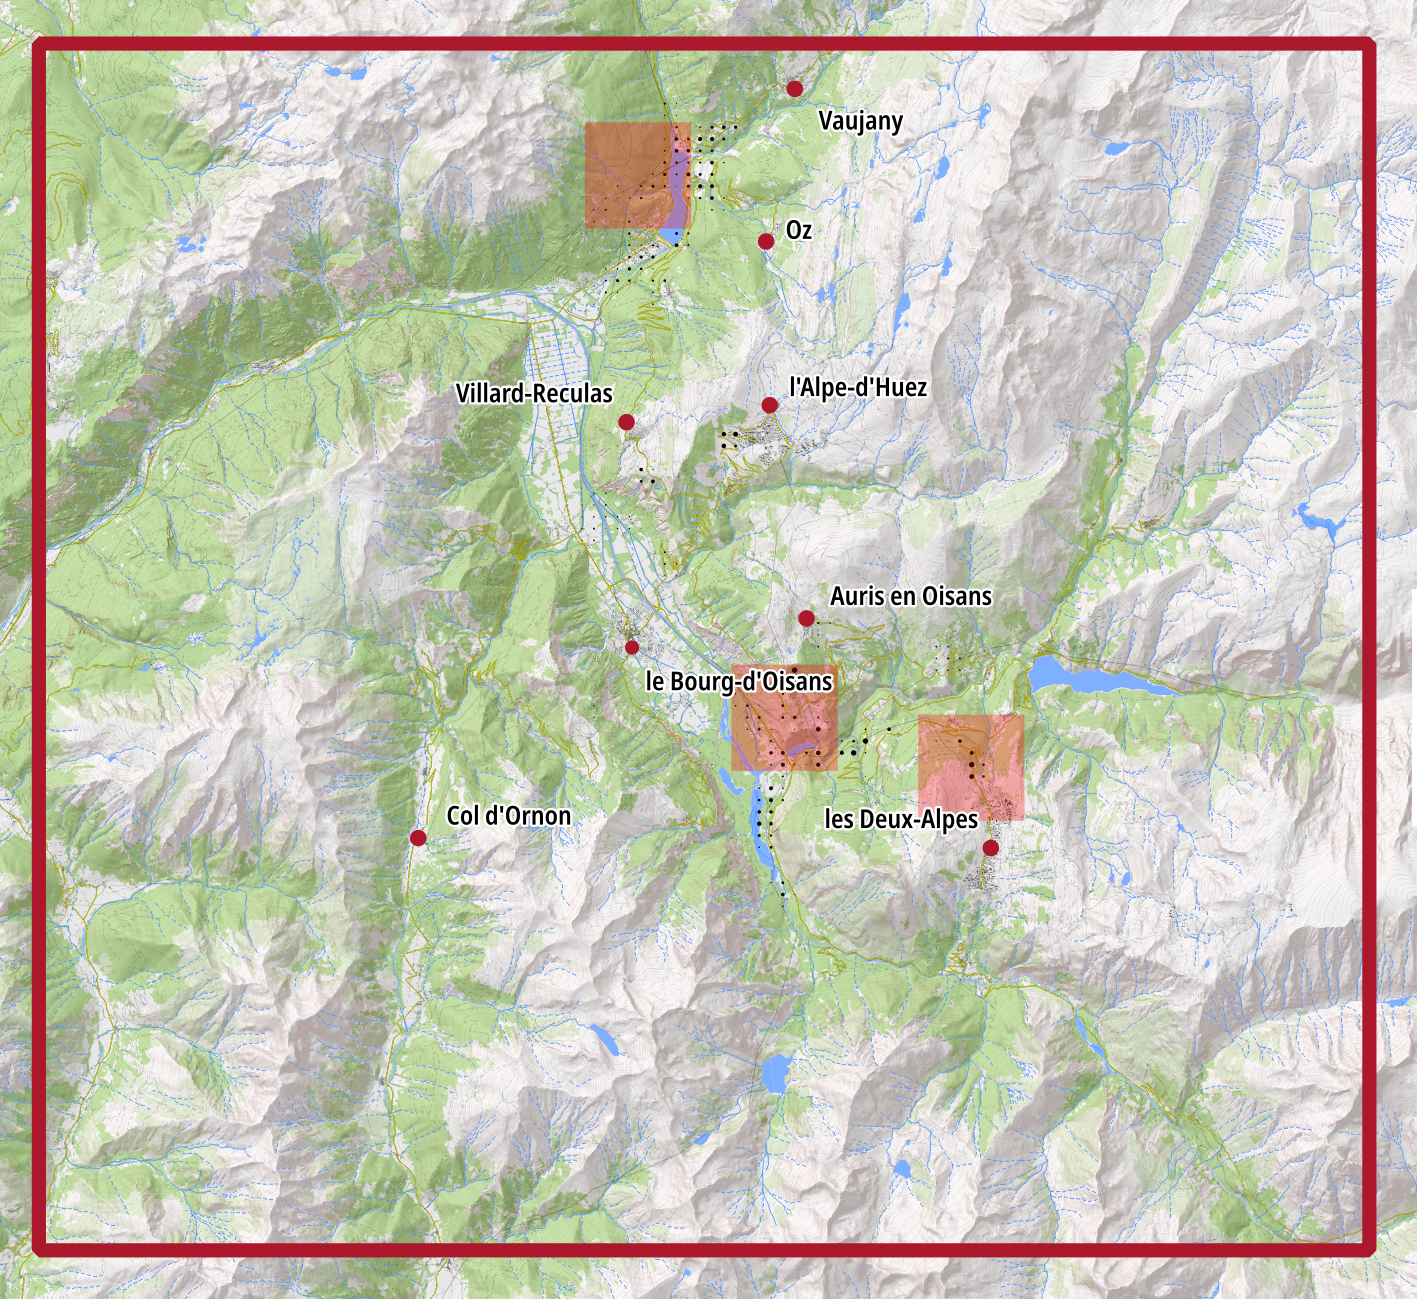
\includegraphics[width=\linewidth]{../figures/ZLP_FilRouge/ZLP.png}};
      \begin{scope}[x=(img.south east),y=(img.north west)]
        \node[draw,minimum height=1.6cm,minimum width=1.00cm] (B1) at (0.2,0.60) {};
        \node[draw,minimum height=0.8cm,minimum width=0.50cm] (B2) at (0.7,0.25) {};
        \node[draw,minimum height=0.4cm,minimum width=0.25cm] (B3) at (0.9,0.10) {};
      \end{scope}
    \end{tikzpicture}
  }
  
  \subfloat[]{%
    \begin{tikzpicture}[remember picture]
      \node (img1) {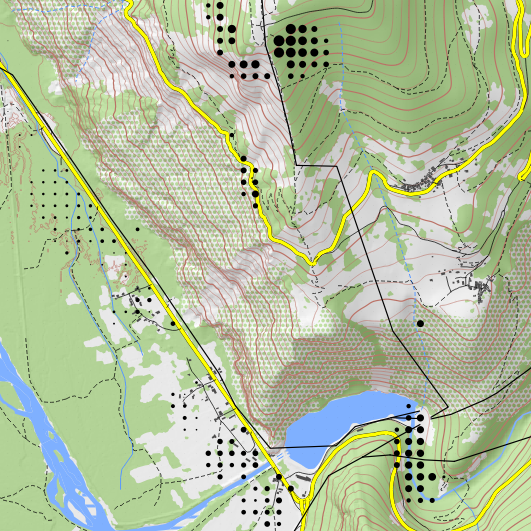
\includegraphics{../figures/ZLP_FilRouge/ZLP_2.png}};
      \draw (img1.south west) rectangle (img1.north east);
    \end{tikzpicture}
  }\hfill
  \subfloat[]{%
    \begin{tikzpicture}[remember picture]
      \node (img2) {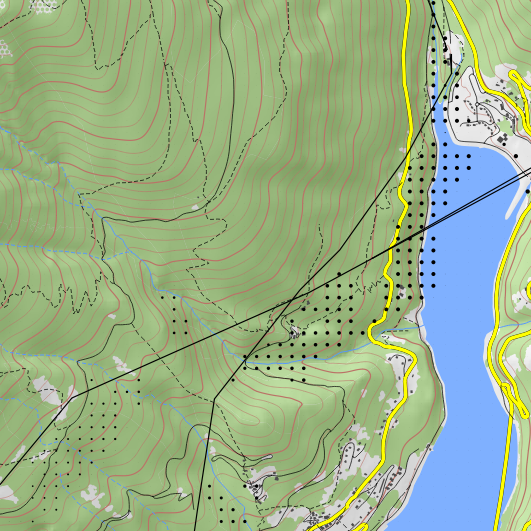
\includegraphics{../figures/ZLP_FilRouge/ZLP_3.png}};
      \draw (img2.south west) rectangle (img2.north east);
    \end{tikzpicture}
  }\hfill
  \subfloat[]{%
    \begin{tikzpicture}[remember picture]
      \node (img3) {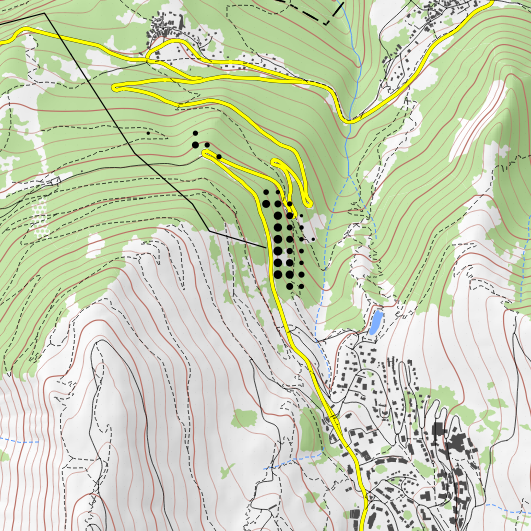
\includegraphics{../figures/ZLP_FilRouge/ZLP_4.png}};
      \draw (img3.south west) rectangle (img3.north east);
    \end{tikzpicture}
  }
  \begin{tikzpicture}[overlay, remember picture]
    \draw (B1) -- (img1);
    \draw (B2) -- (img2);
    \draw (B3) -- (img3);
  \end{tikzpicture}